\section{数据观察}
\label{sec:observation}

由于我们参加比赛的时候,比赛已经进行了大约8个月,Kaggle上已经有了较多公开的脚本。在这一节的分析中,一些可视化结果是参考了公开发布的脚本做出来的。值得说明的是,除了本节之外,第\ref{sec:feature}节中提到的所有数据处理和第\ref{sec:model}节中使用的模型都是我们独立实现的脚本,没有参考其他任何来源的资料。

\subsection{犯罪总量分析}

在这一小节,我们对数据集进行粗粒度的分析。即,只变化数据点的某一个字段,而对其他字段的全体可能取值统计总数,观察每个字段的取值对于犯罪总体情况的影响。所谓犯罪总体情况,就是忽略犯罪类型,关注犯罪案件的总数。这部分分析看似并不能帮助我们进行分类,但是可以先帮我们从一个比较宏观的角度看时间和地点是如何影响犯罪的。站在实际应用角度,从时间、地点等侧面统计总体犯罪情况,可以作为当地警察局部署警力的有益参考。

\begin{figure}[tb]
    \centering
    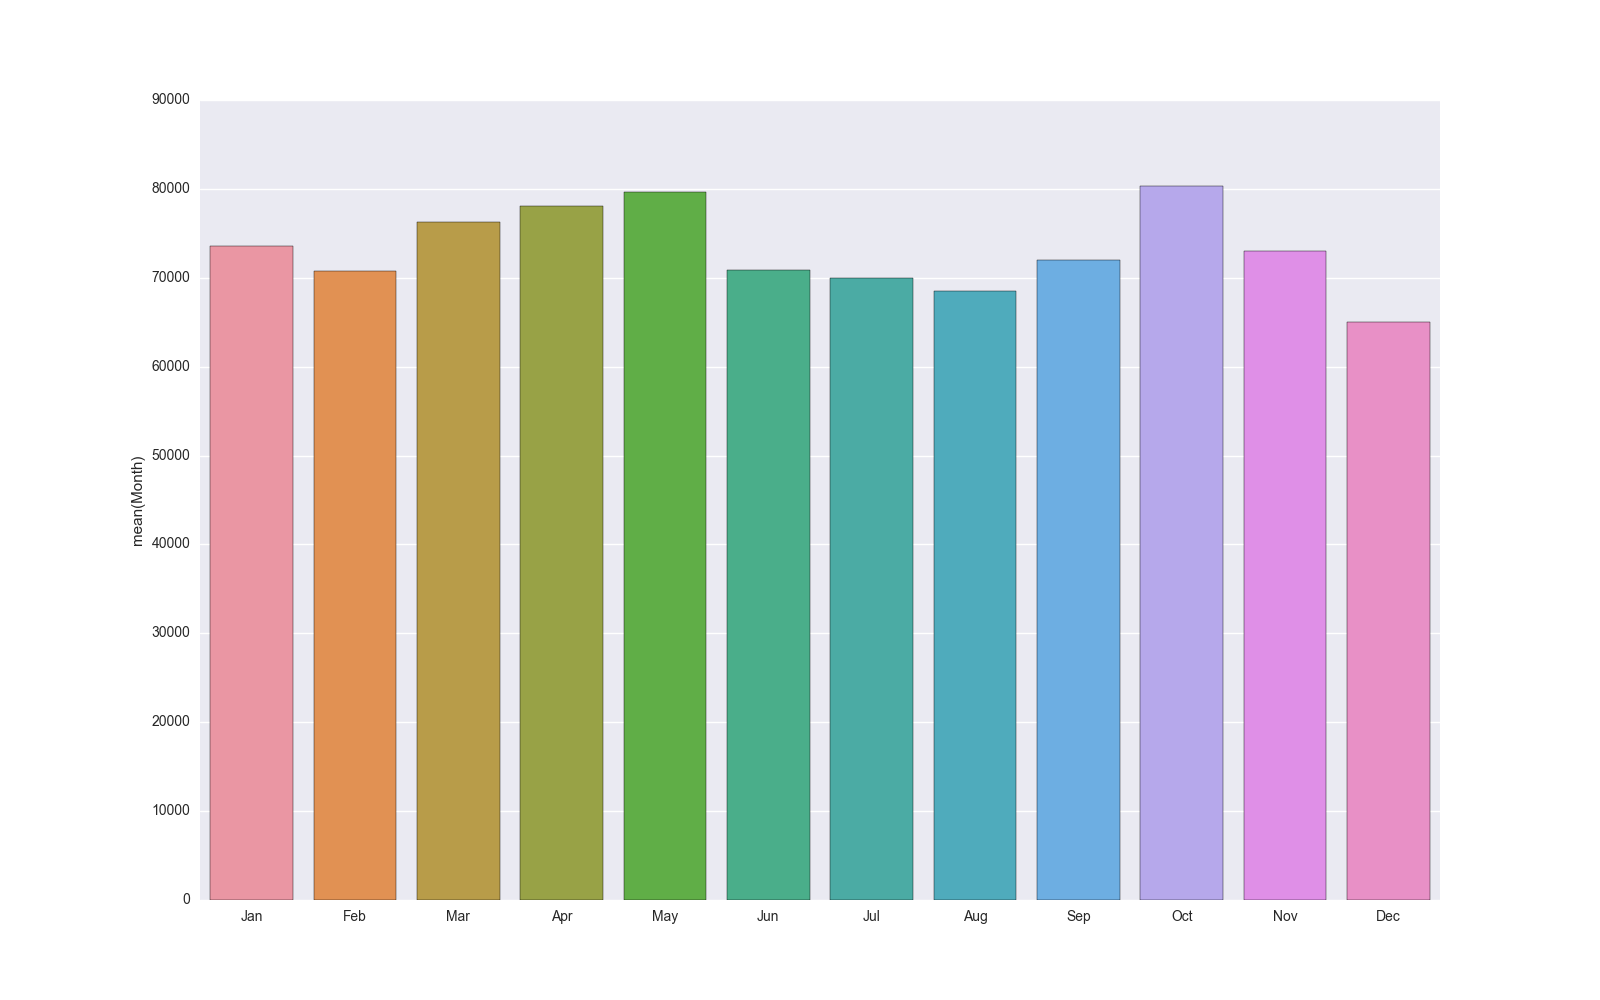
\includegraphics[width=1.0\linewidth]{fig/monthly}
    \caption{月份对犯罪总量的影响}
    \label{fig:monthly}
\end{figure}

\begin{figure}[tb]
    \centering
    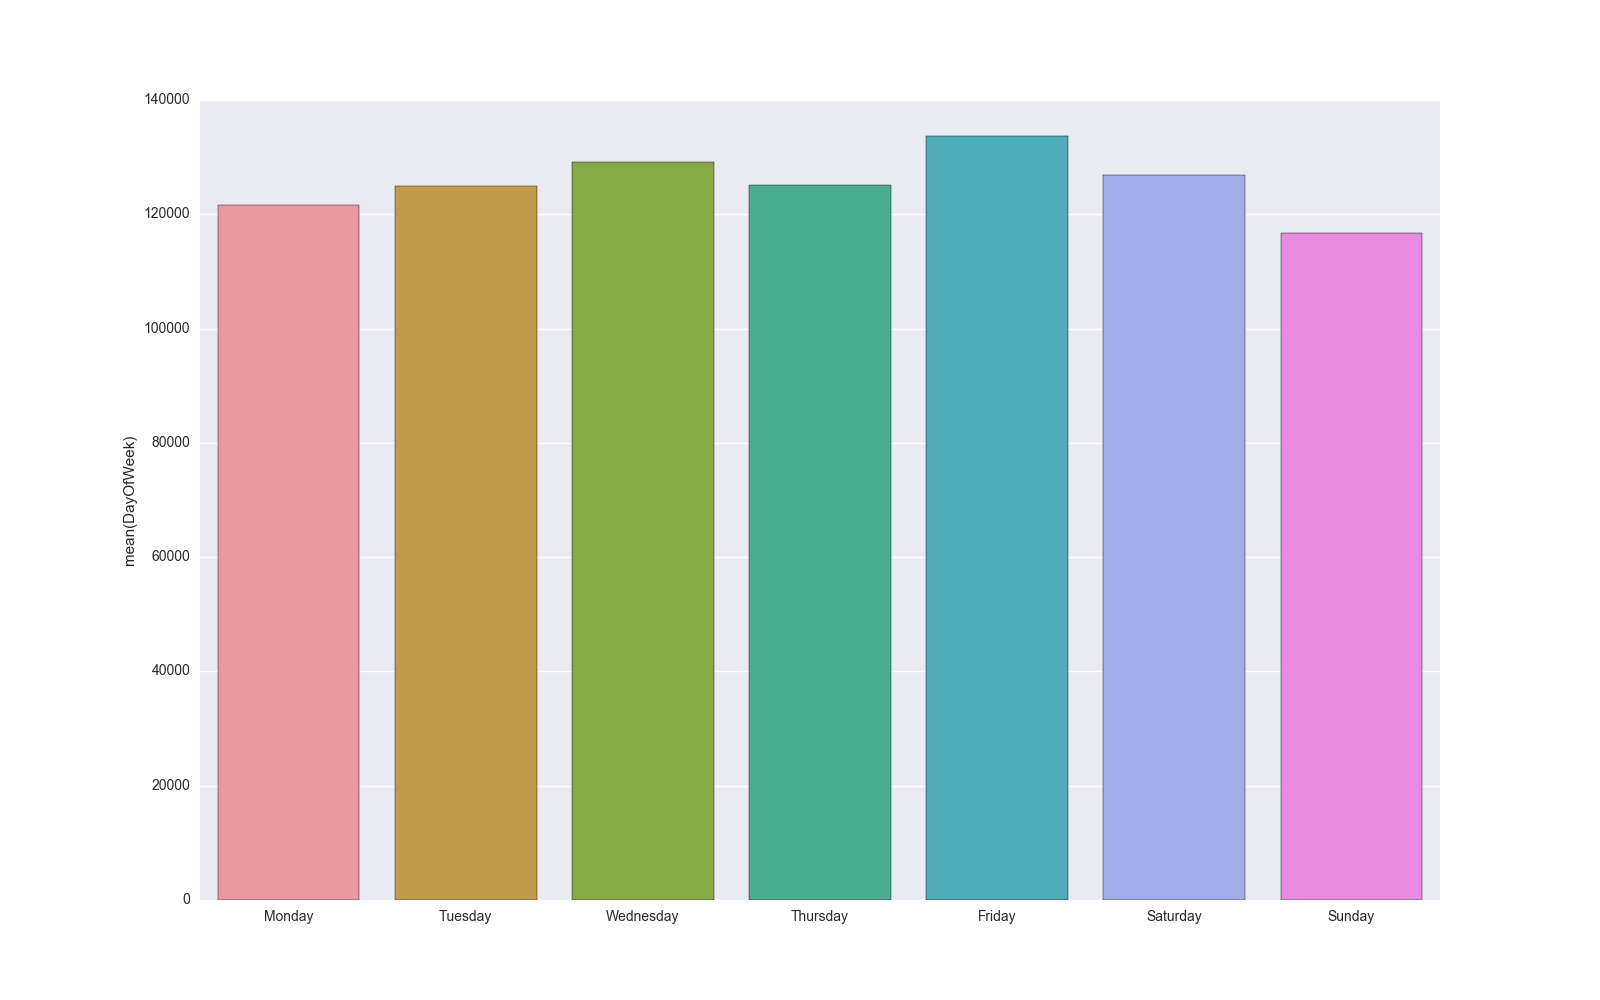
\includegraphics[width=1.0\linewidth]{fig/DayOfWeek}
    \caption{星期对犯罪总量的影响}
    \label{fig:dayofweek}
\end{figure}

\begin{figure}[tb]
    \centering
    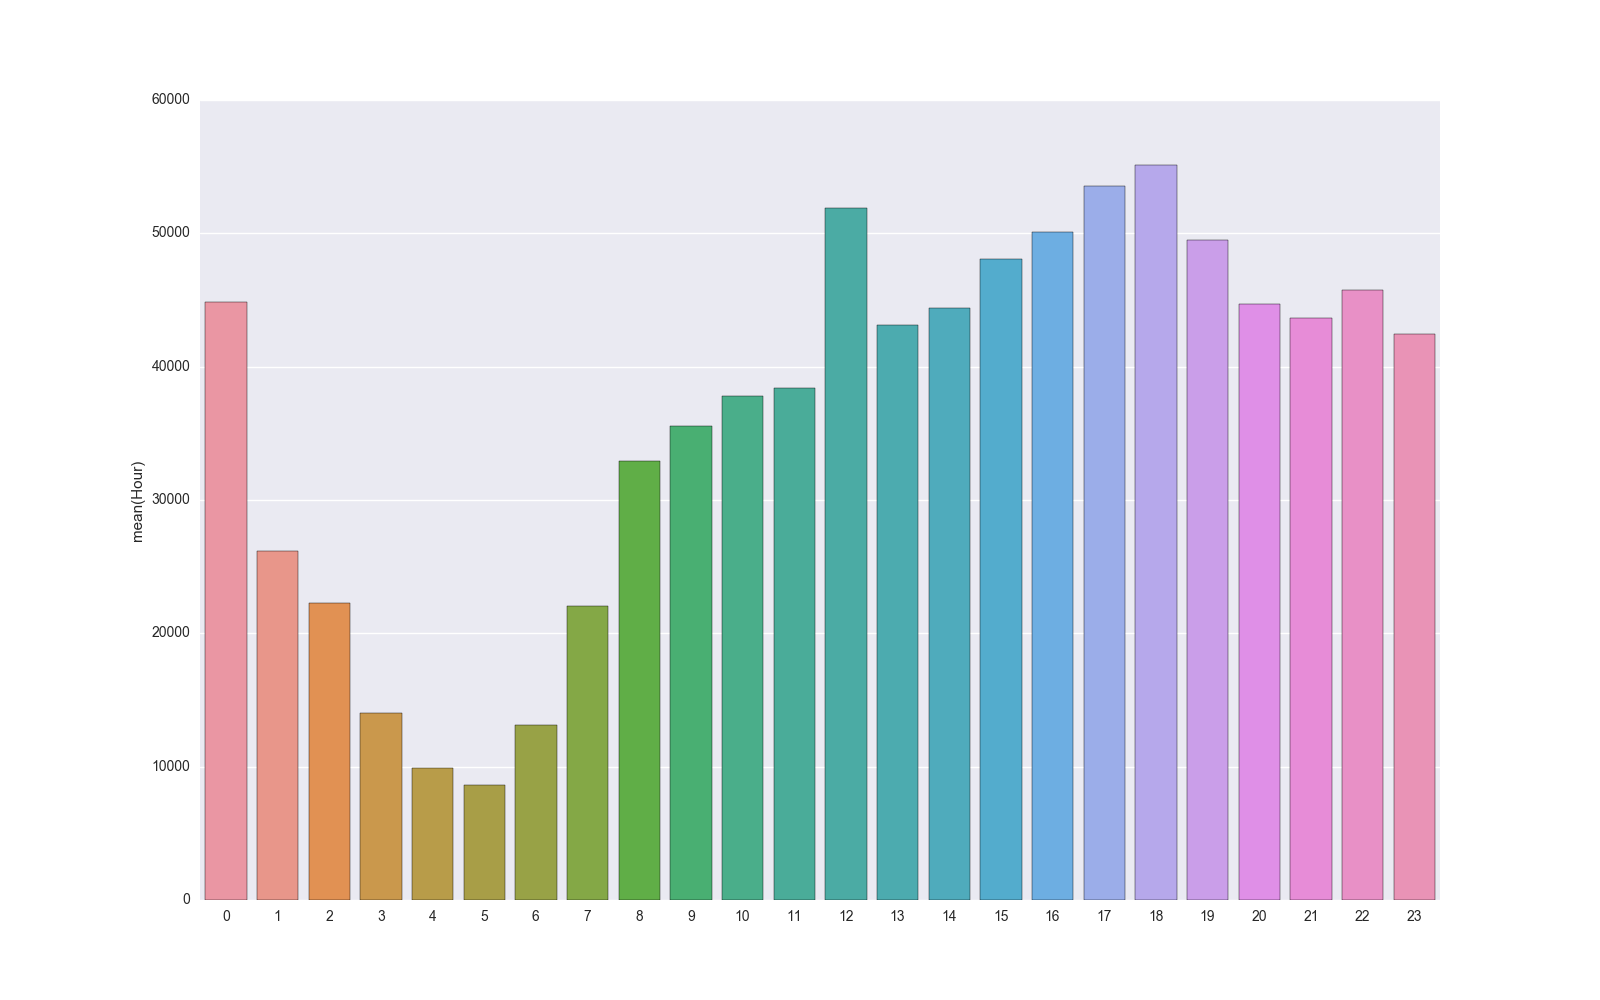
\includegraphics[width=1.0\linewidth]{fig/Hourly}
    \caption{小时对犯罪总量的影响}
    \label{fig:hourly}
\end{figure}

图\ref{fig:monthly}、图\ref{fig:dayofweek}和图\ref{fig:hourly}分别展示了月份、星期和小时对犯罪总量的影响。可见,月份变化时,犯罪总量会发生比较明显的起伏波动,但相比之下,每周的每一天的犯罪总量的变化则不那么明显。符合预期的是,小时对于犯罪的影响是最显著的:中午、傍晚和午夜有三个比较明显的犯罪高峰,而凌晨的犯罪则比较少,这一分布情况用生活经验很容易理解。

\begin{figure}[tb]
    \centering
    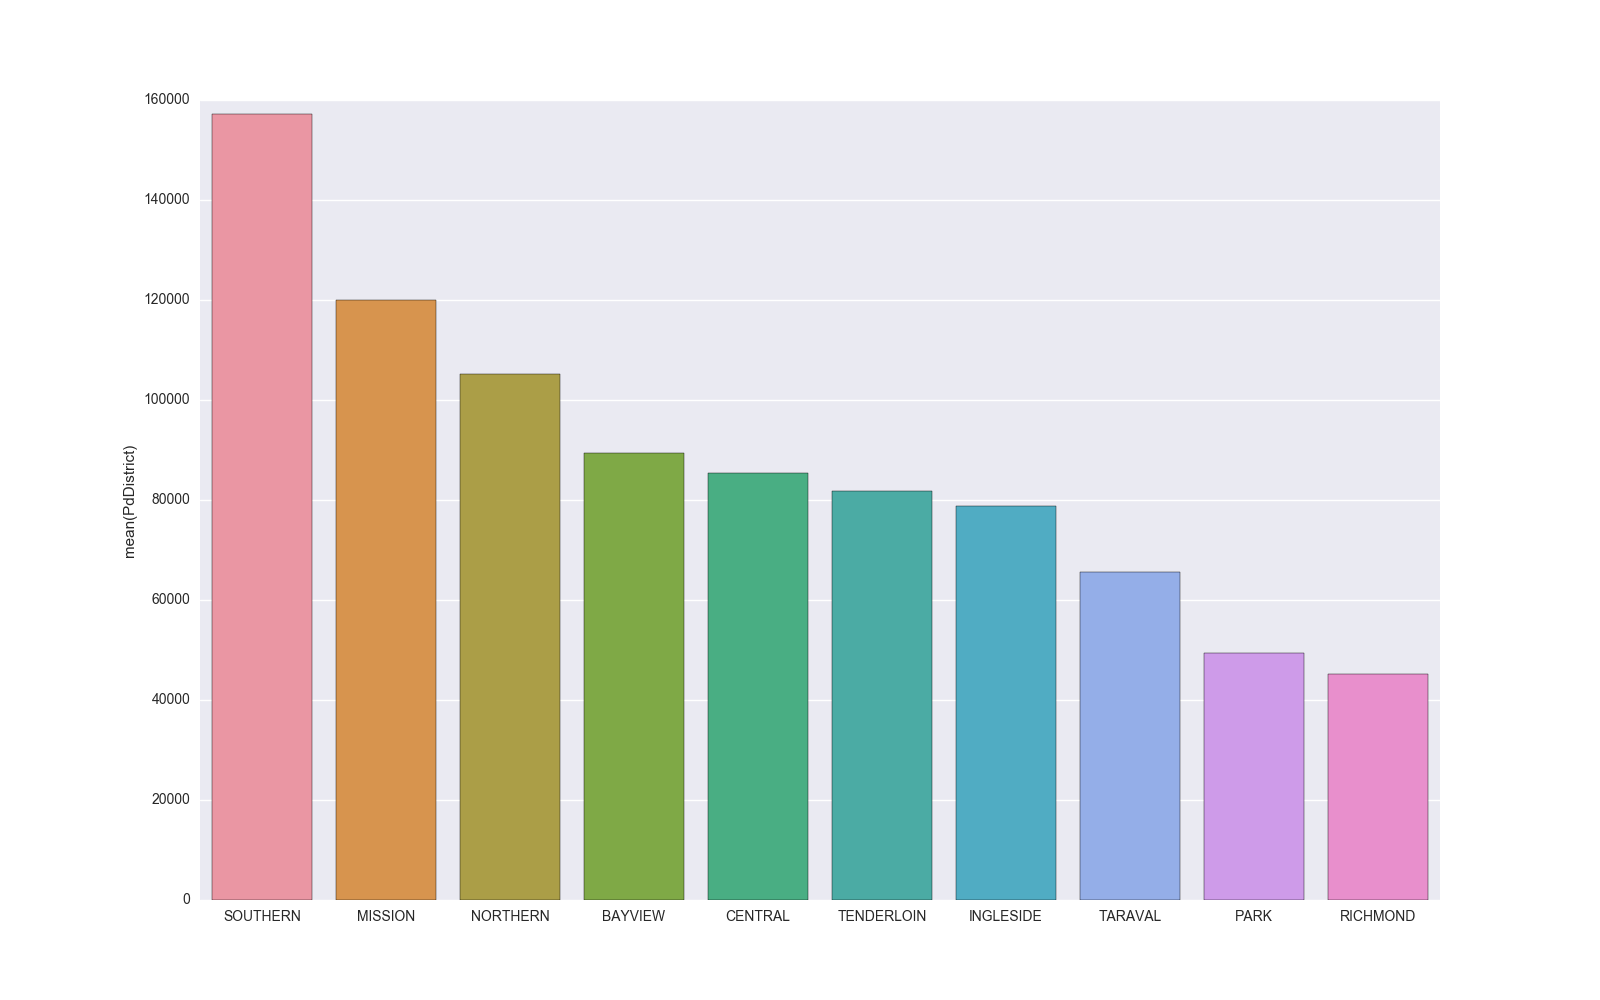
\includegraphics[width=1.0\linewidth]{fig/PdDistrict}
    \caption{各警察局片区的犯罪总量影响}
    \label{fig:pd_district}
\end{figure}

\begin{figure}[tb]
    \centering
    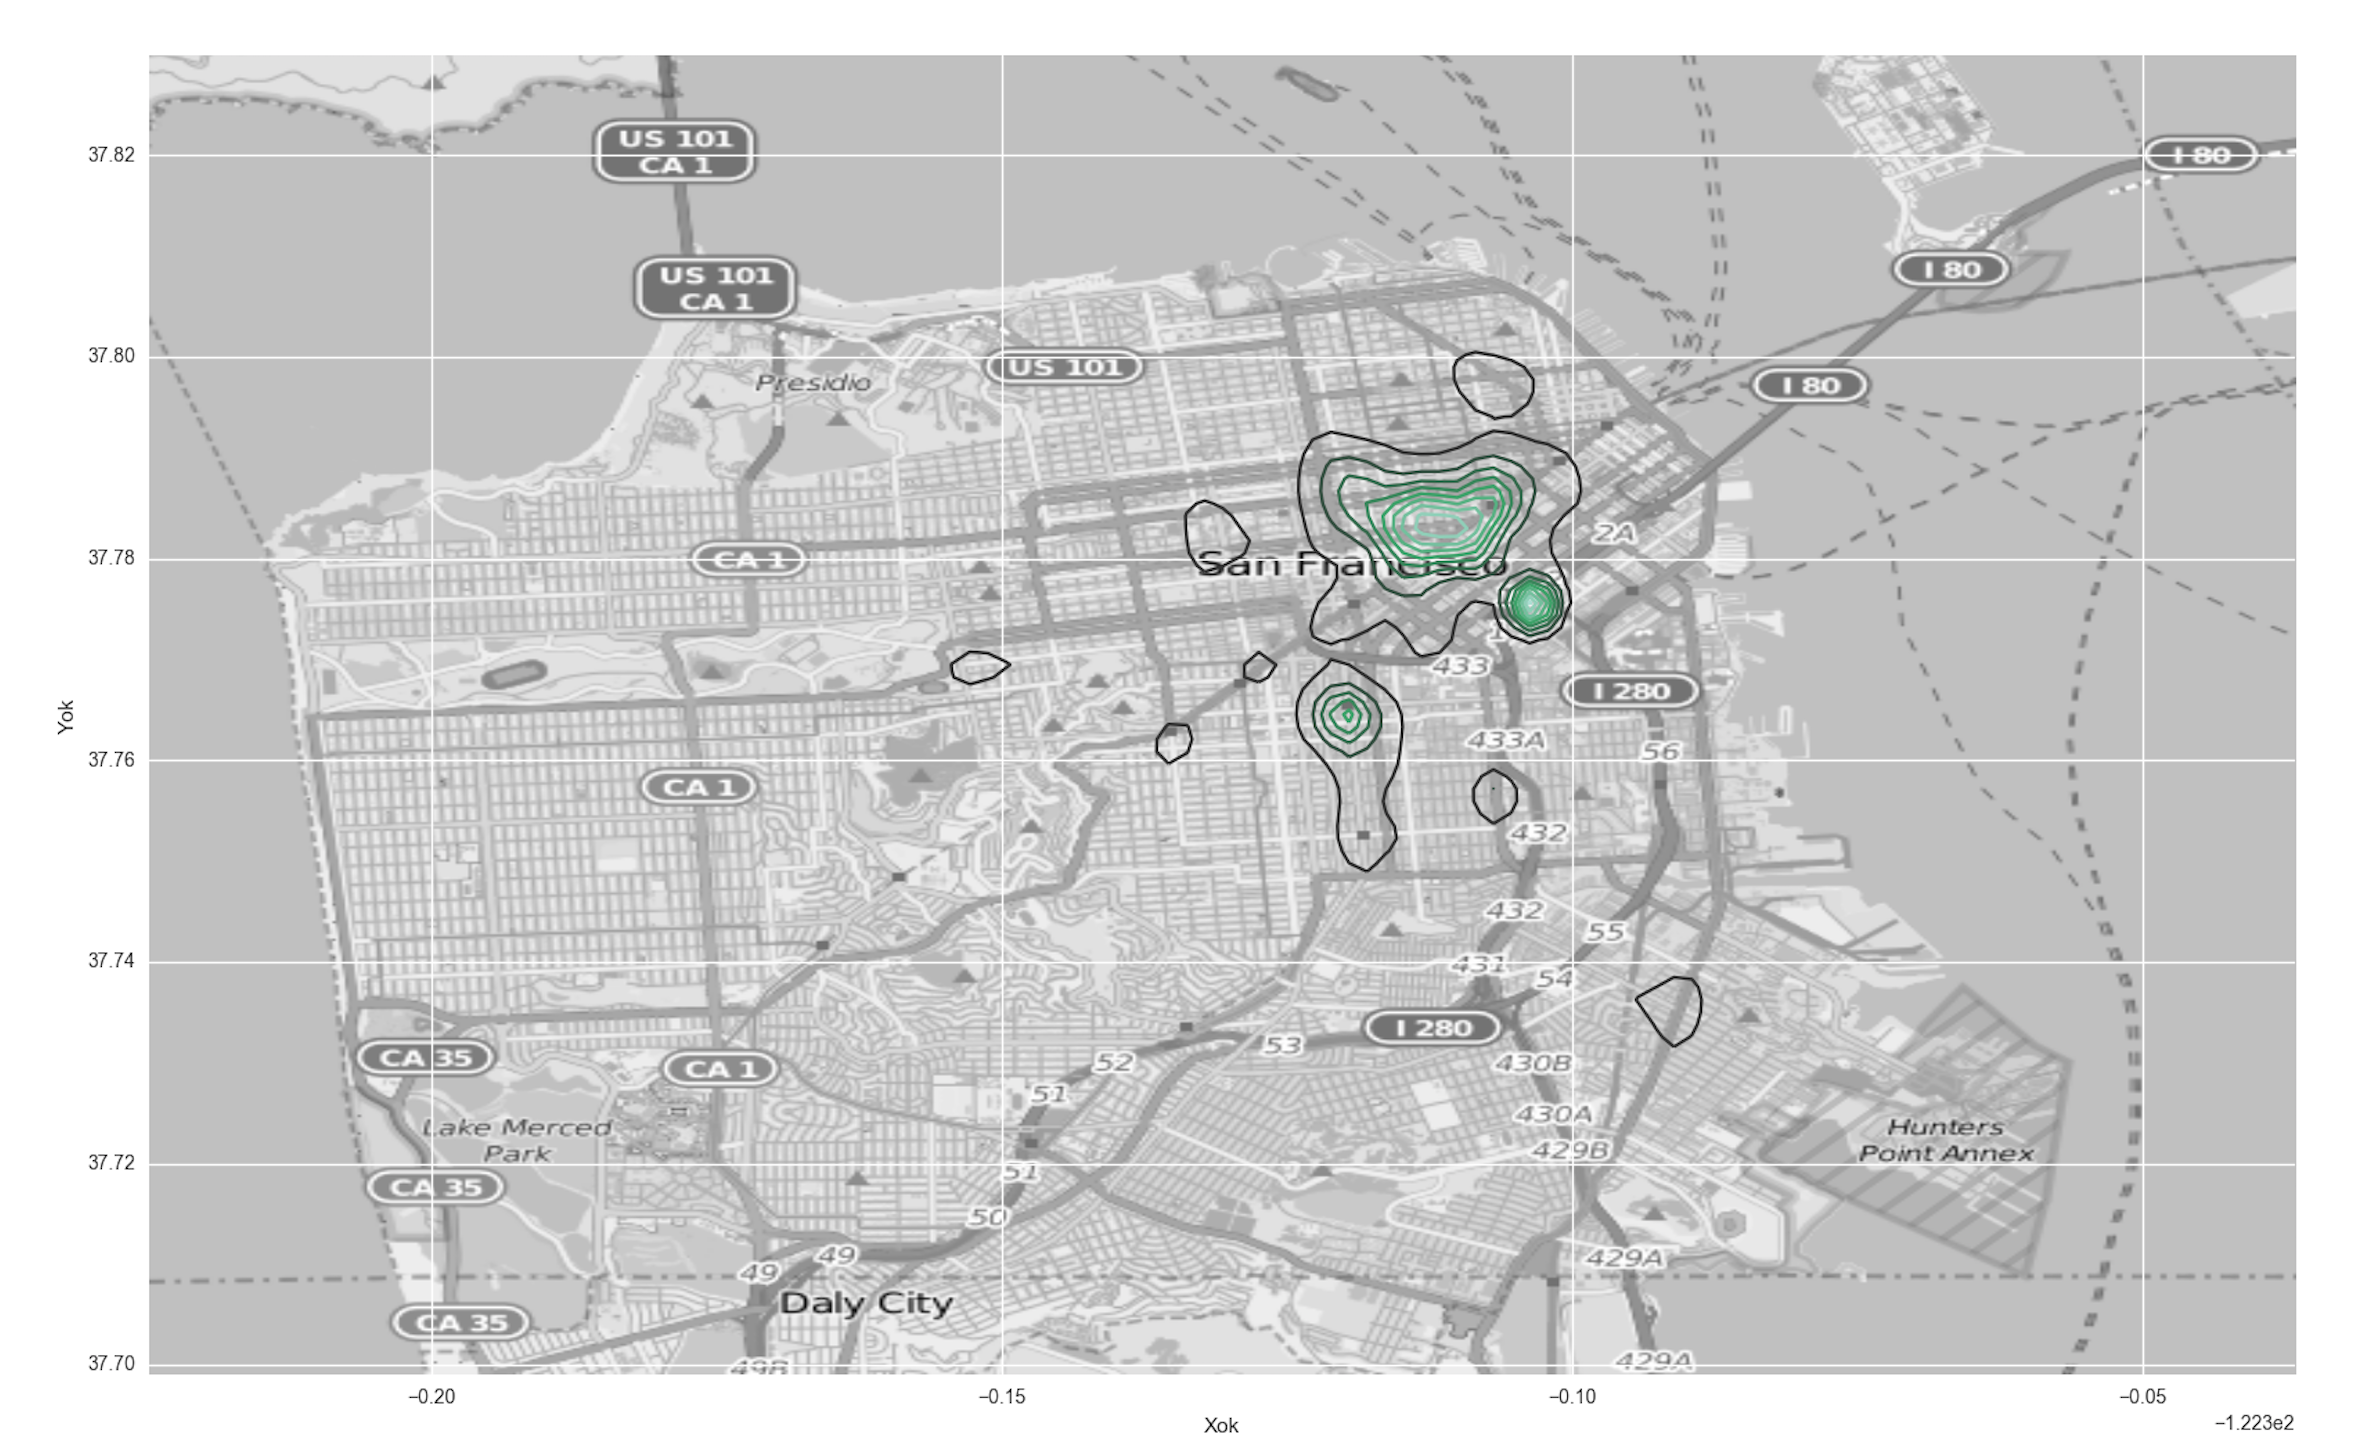
\includegraphics[width=1.0\linewidth]{fig/total_density}
    \caption{犯罪总量的热度图}
    \label{fig:tot_density}
\end{figure}

下面观察不同地点对犯罪总量的影响。首先,由图\ref{fig:pd_district}可以看出,不同警察局区域的犯罪量的差异是巨大的。由此可以推断出城市不同区域的犯罪率有巨大的不同。作为验证,我们参考Kaggle上公开的一份代码\footnote{https://www.kaggle.com/codechamp/sf-crime/crime-density-by-location/code,作者codechamp},对全部类型的犯罪总量做密度图,即图\ref{fig:tot_density}。从中可以看出,城市东北角的犯罪率要显著高于其他部分。

\subsection{犯罪类型分布的分析}

\begin{figure}[tb]
    \centering
    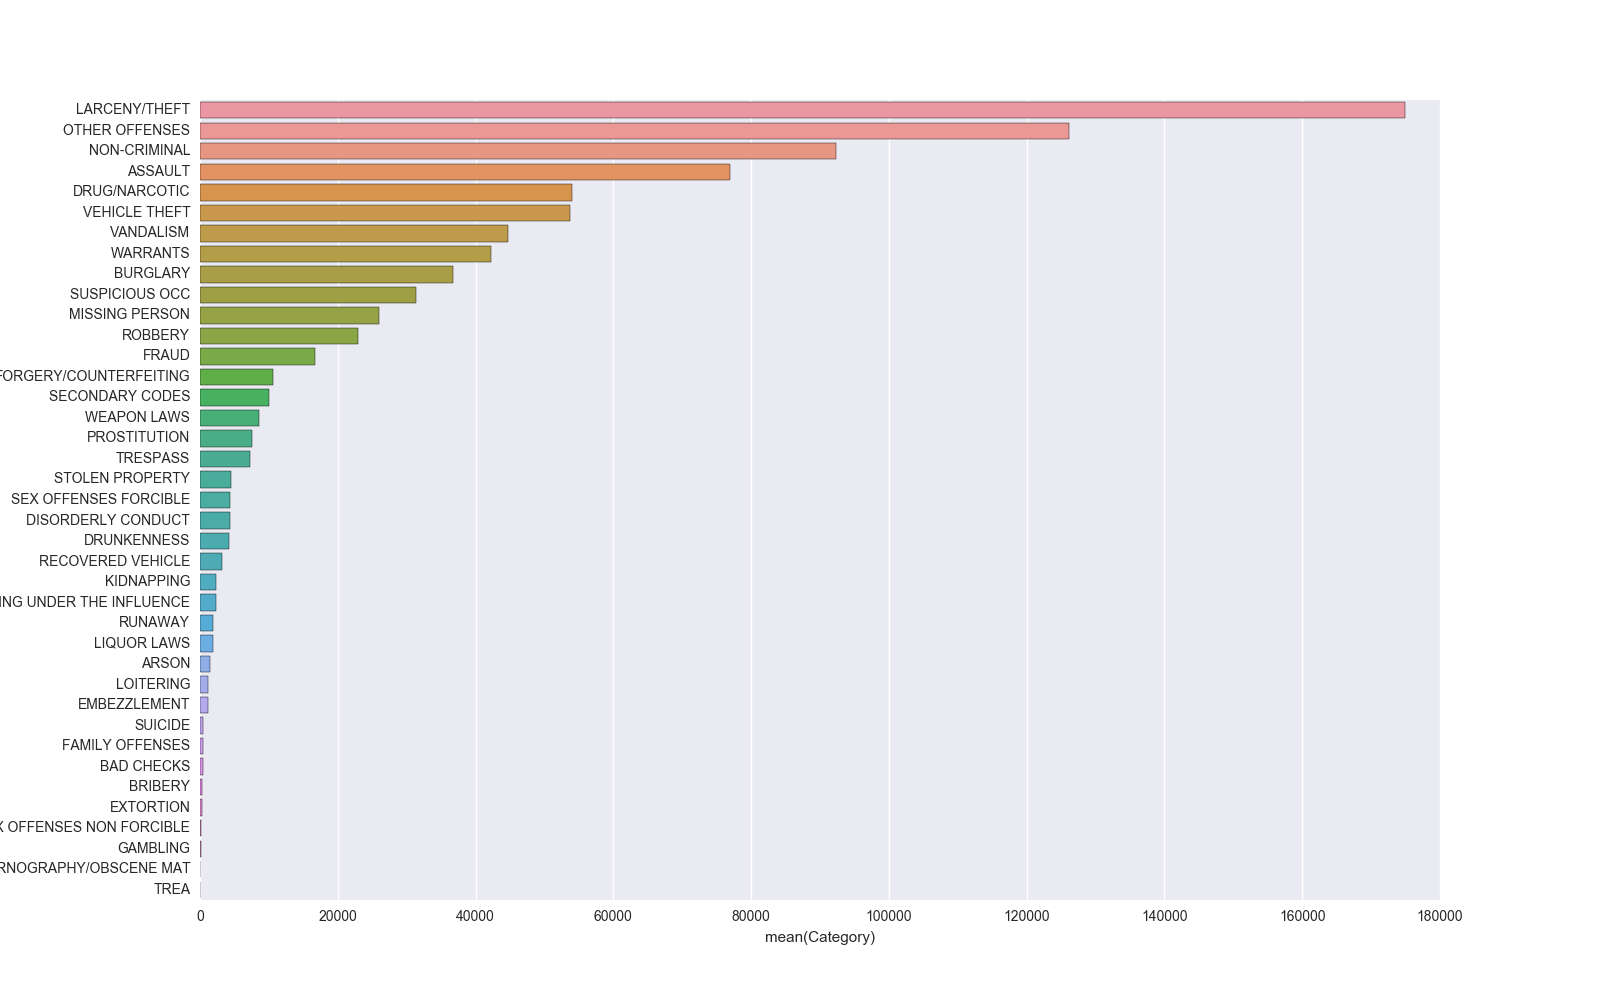
\includegraphics[width=1.0\linewidth]{fig/category}
    \caption{不同犯罪类型的总量}
    \label{fig:tot_category}
\end{figure}

首先,我们先不区分时间和地点,考察总体上各种犯罪类型的分布。图\ref{fig:tot_category}中可见,不同类型的犯罪总量是一个长尾分布,即频数最高的几个犯罪类型的总量占到了总体犯罪总数的大部分(最多的5种犯罪占整体犯罪总数的66\%)。由此可以推知,有些犯罪类型的概率总是很高的,即便一些长尾类型在某个地点集中,它的概率可能仍然没有常见类型的概率大。这种情形将会对我们的预测带来一些困难。下面,带着对犯罪类型分布的总体认识,我们进一步从地点、时间角度进行一些分析,并进一步对时间做出限制进行细粒度分析。

\subsubsection{不同犯罪类型对地点的分布}

图\ref{fig:tot_density}中已经看到了犯罪总量对于地点的分布,发现犯罪整体上趋向于同一个中心。如果每一种犯罪类型单独分析时,都趋向于这个中心,那么可以认为地点对于每种犯罪类型的概率的影响是一致的,即地点信息对于预测犯罪类型没有任何帮助。但是,图\ref{fig:tot_category}中的结果可以看到,虽然绝大多数犯罪类型都会有城市东北角的密度中心,很多犯罪类型也会有其他的密度中心。比如,纵火(ARSON)和赌博(GAMBLING)都在城市的东南角有一个密度中心。更有趣的是一个例子是,离家出走(RUNAWAY)的密度中心和其他任何一种犯罪类型的都十分不同,这应该是源于“离家出走”其实并不是真正的犯罪。总之,根据图\ref{fig:tot_category},不同犯罪类型在地点上的分布是有所不同的,所以地点信息对预测很有帮助。另外值得注意的是,频率最高的几种犯罪类型:盗窃(THEFT)、其他侵犯(OTHER OFFENSES)、无罪(NON-CRIMINAL)、攻击(ASSAULT)、吸毒(DRUG)的密度中心都集中在城市东北角,即全部犯罪类型的集中位置。也就是说,对于高频犯罪,地点信息的辨别能力不强。

\begin{figure*}[!bt]
    \centering
    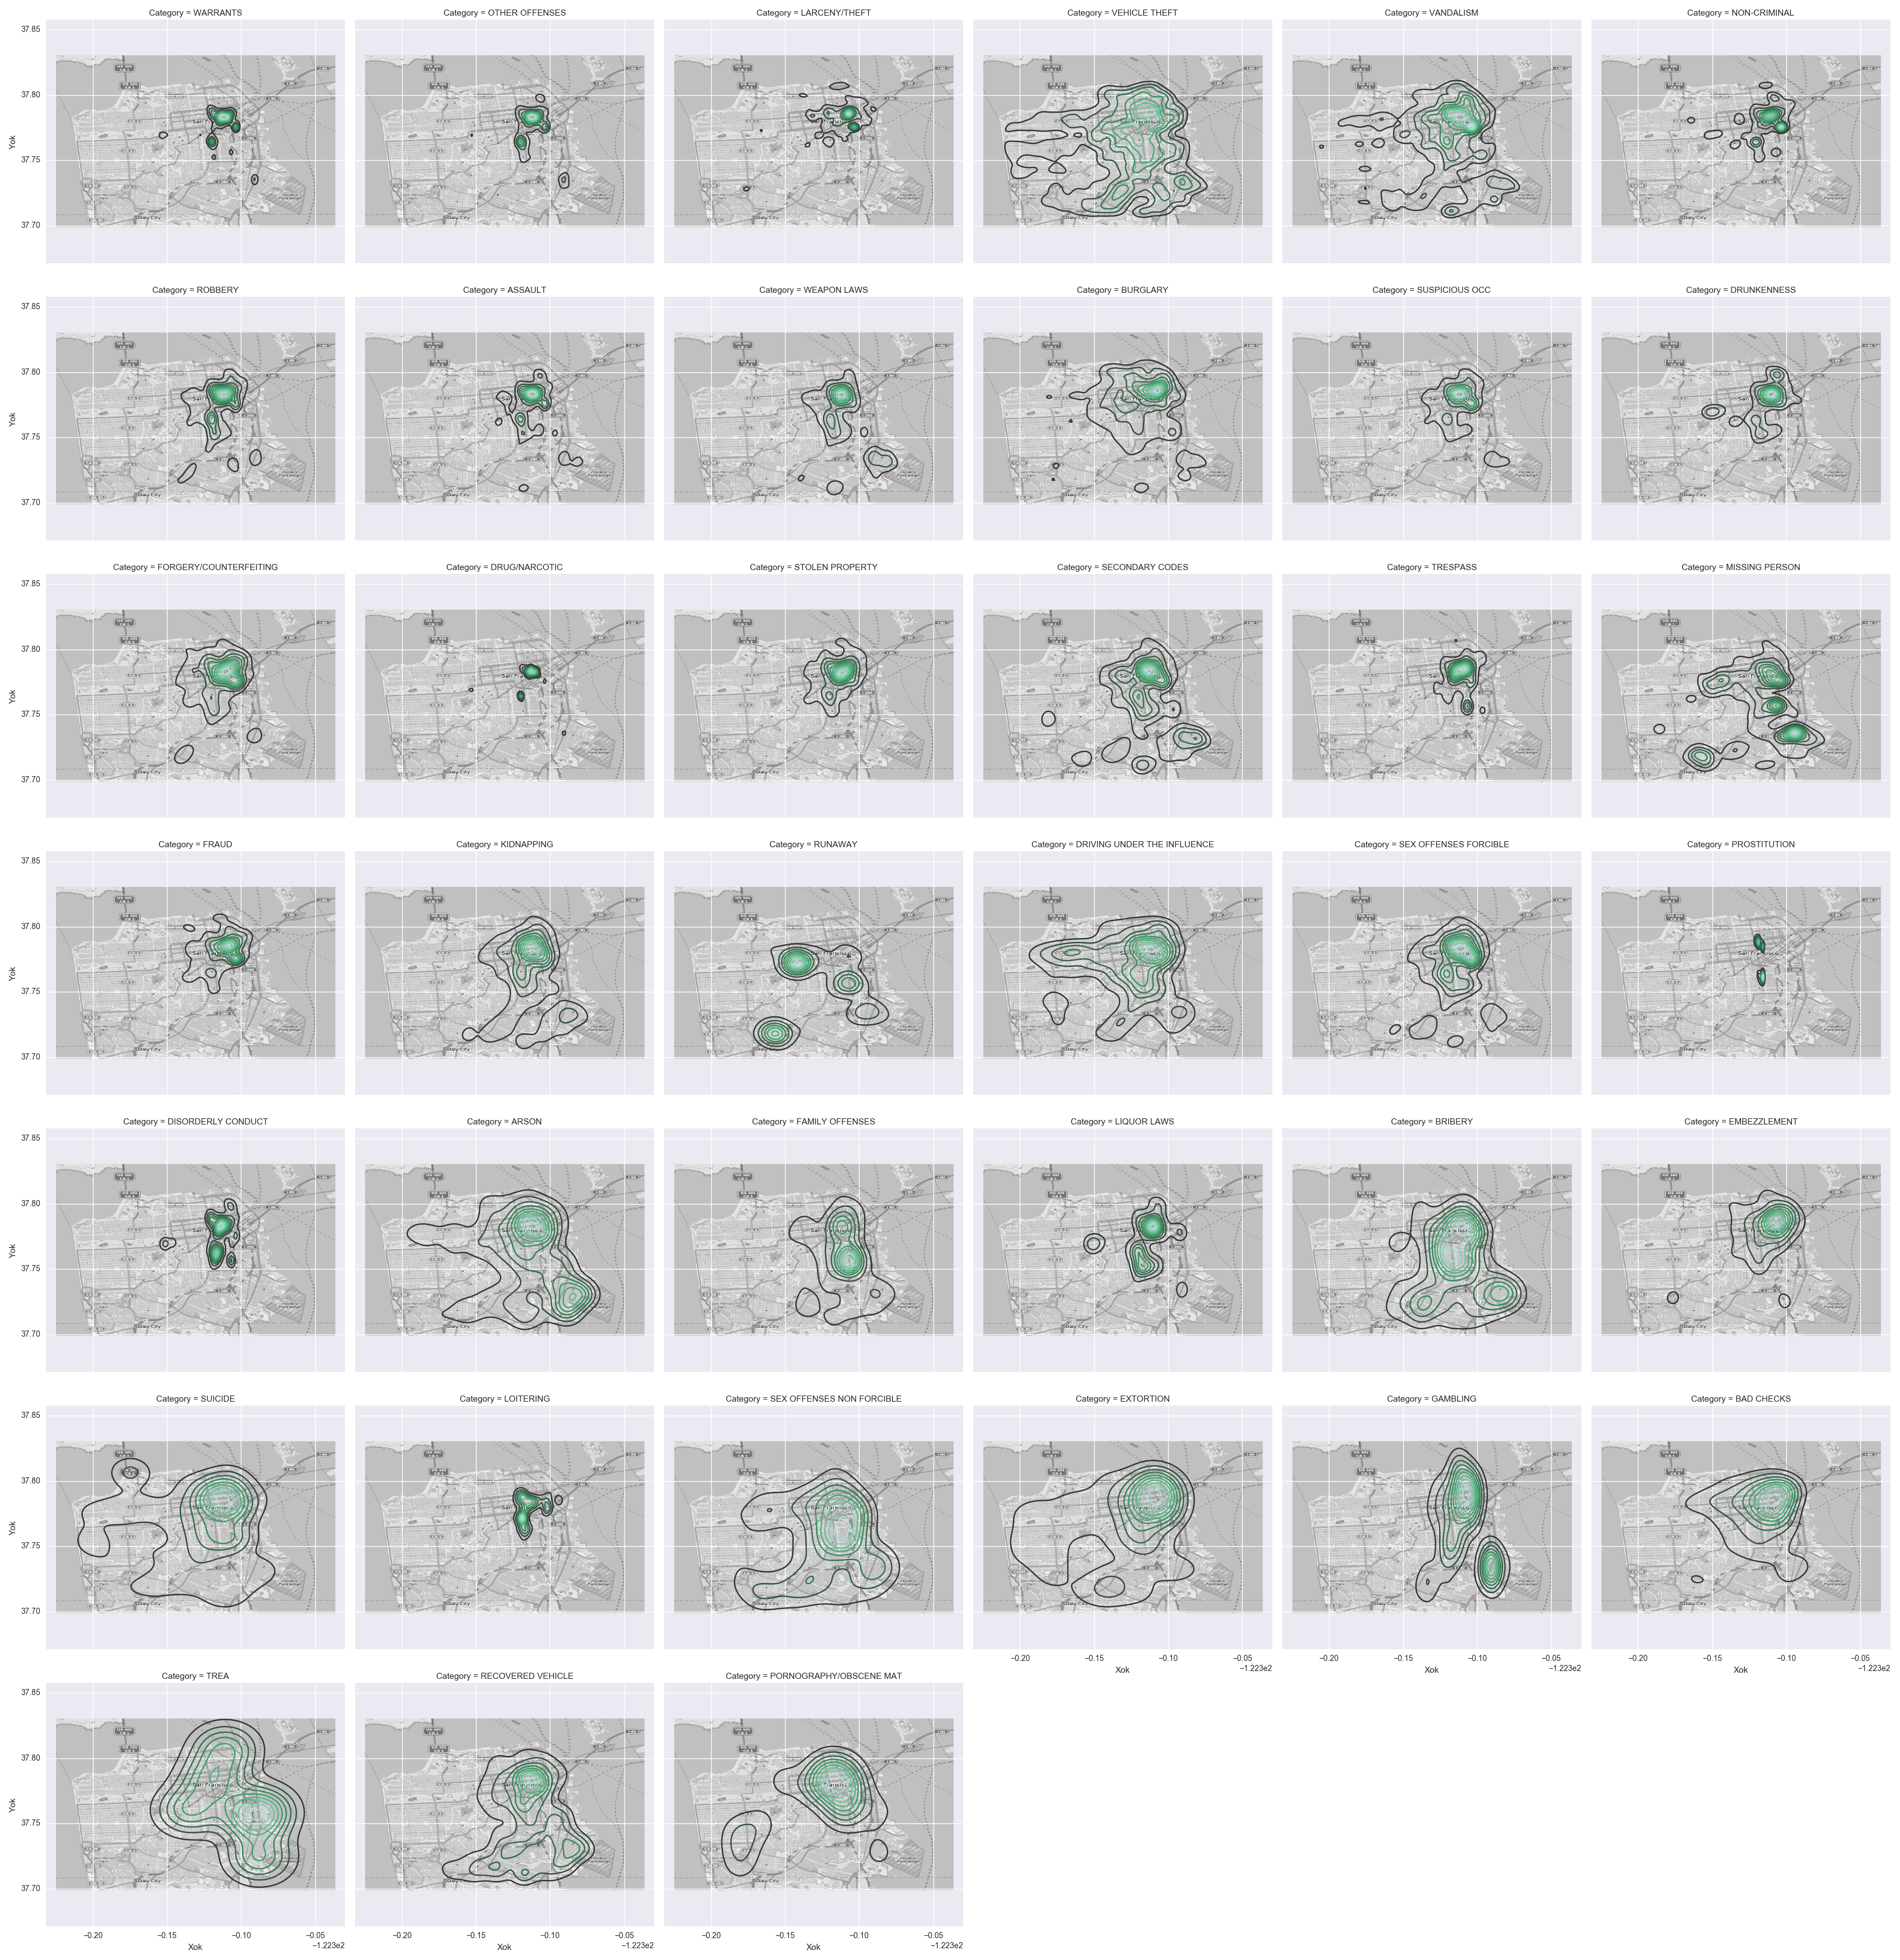
\includegraphics[width=1.0\linewidth]{fig/category_density}
    \caption{每种犯罪类型的密度图}
    \label{fig:tot_category}
\end{figure*}

\newpage

\subsubsection{不同犯罪类型对时间的分布}

对于时间分布的分析,我们采用的方法是比较不同时间特征下,犯罪分布的相似程度。对于离散分布的相似性比较,我们使用的方法是计算两个分布的相关系数:

\begin{equation*}
r_{xy}=\frac{\sum^n_{i=1}(x_i-\bar{x})(y_i-\bar{y})}{\sqrt{\sum^n_{i=1}(x_i-\bar{x})^2\sum^n_{i=1}(y_i-\bar{y})^2}}
\end{equation*}

其中,$x_1, x_2, \dot, x_{39}$表示一个时间特征下的犯罪类型分布(即每种犯罪类型发生的概率);$y_1, y_2, \dot, y_{39}$表示需要比较的另外一个分布。如果两个分布接近,即几乎满足$y_i=x_i$,则线性相关程度较高,计算出的相关系数也会越接近1。否则,如果分布差异很大,则计算出的结果会更接近0。可见,使用相关系数比较离散分布的相似性是合理的。

\begin{figure}[H]
    \centering
    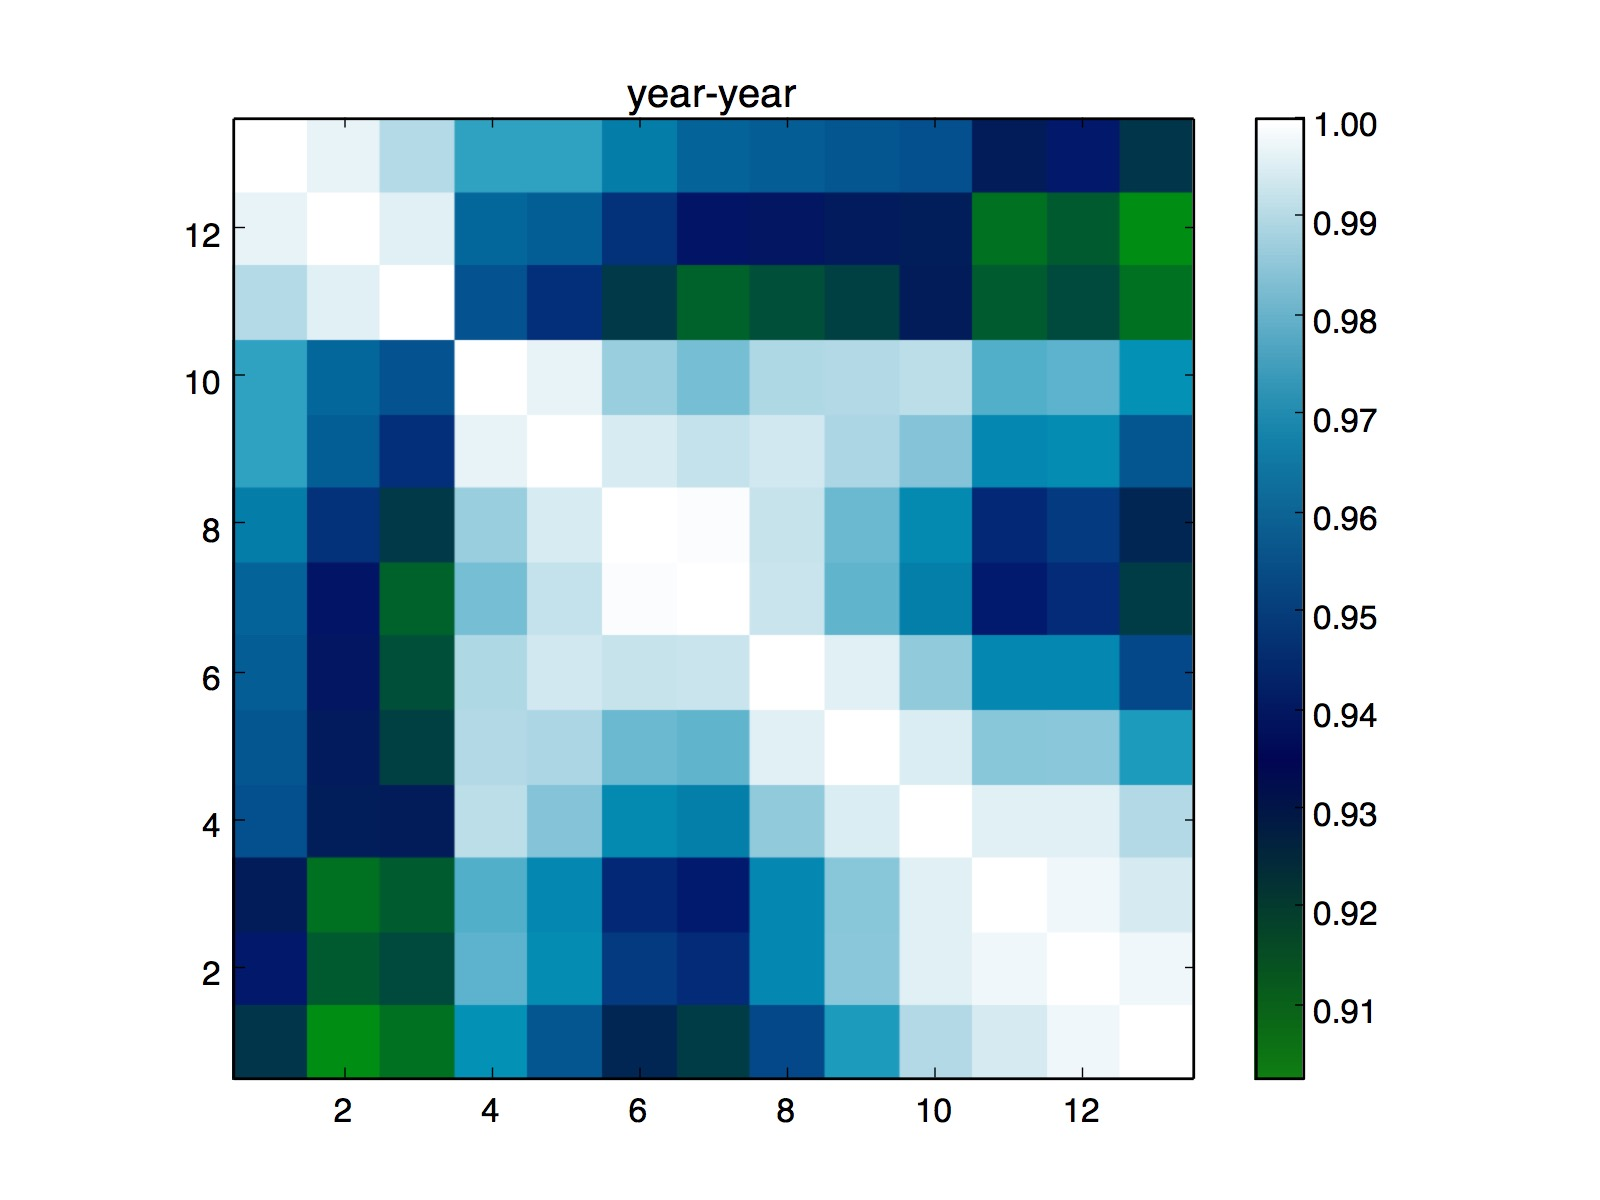
\includegraphics[width=1.0\linewidth]{fig/year_corr}
    \caption{不同年犯罪分布的比较}
    \label{fig:year_corr}
\end{figure}

从图\ref{fig:year_corr}可以看出,不同年份犯罪类型分布还是有一定差异的。特别地,我们看出一个明显的分界,那就是第3年(2005年)和第4年(2006年)之间。前三年的分布比较接近,后就九年的分布比较接近,而这两个时间段之间的差异还是比较大的。图\ref{fig:month_corr}中的结果则表明,不同月份之间的分布相似度都较大(相关系数最小的也有0.992),但是,也可以通过图中对角线的浅色区域看出月份越接近,犯罪分布越接近。图\ref{fig:weekday_corr}中则表明,每周各天的差异也比较小(相关系数至少有0.9855),但是也明显看出周末,即周五、周六、周日的犯罪分布十分接近,而一周中间的周三、周四和其他各天的犯罪分布的差异都比较大。

\begin{figure}[H]
    \centering
    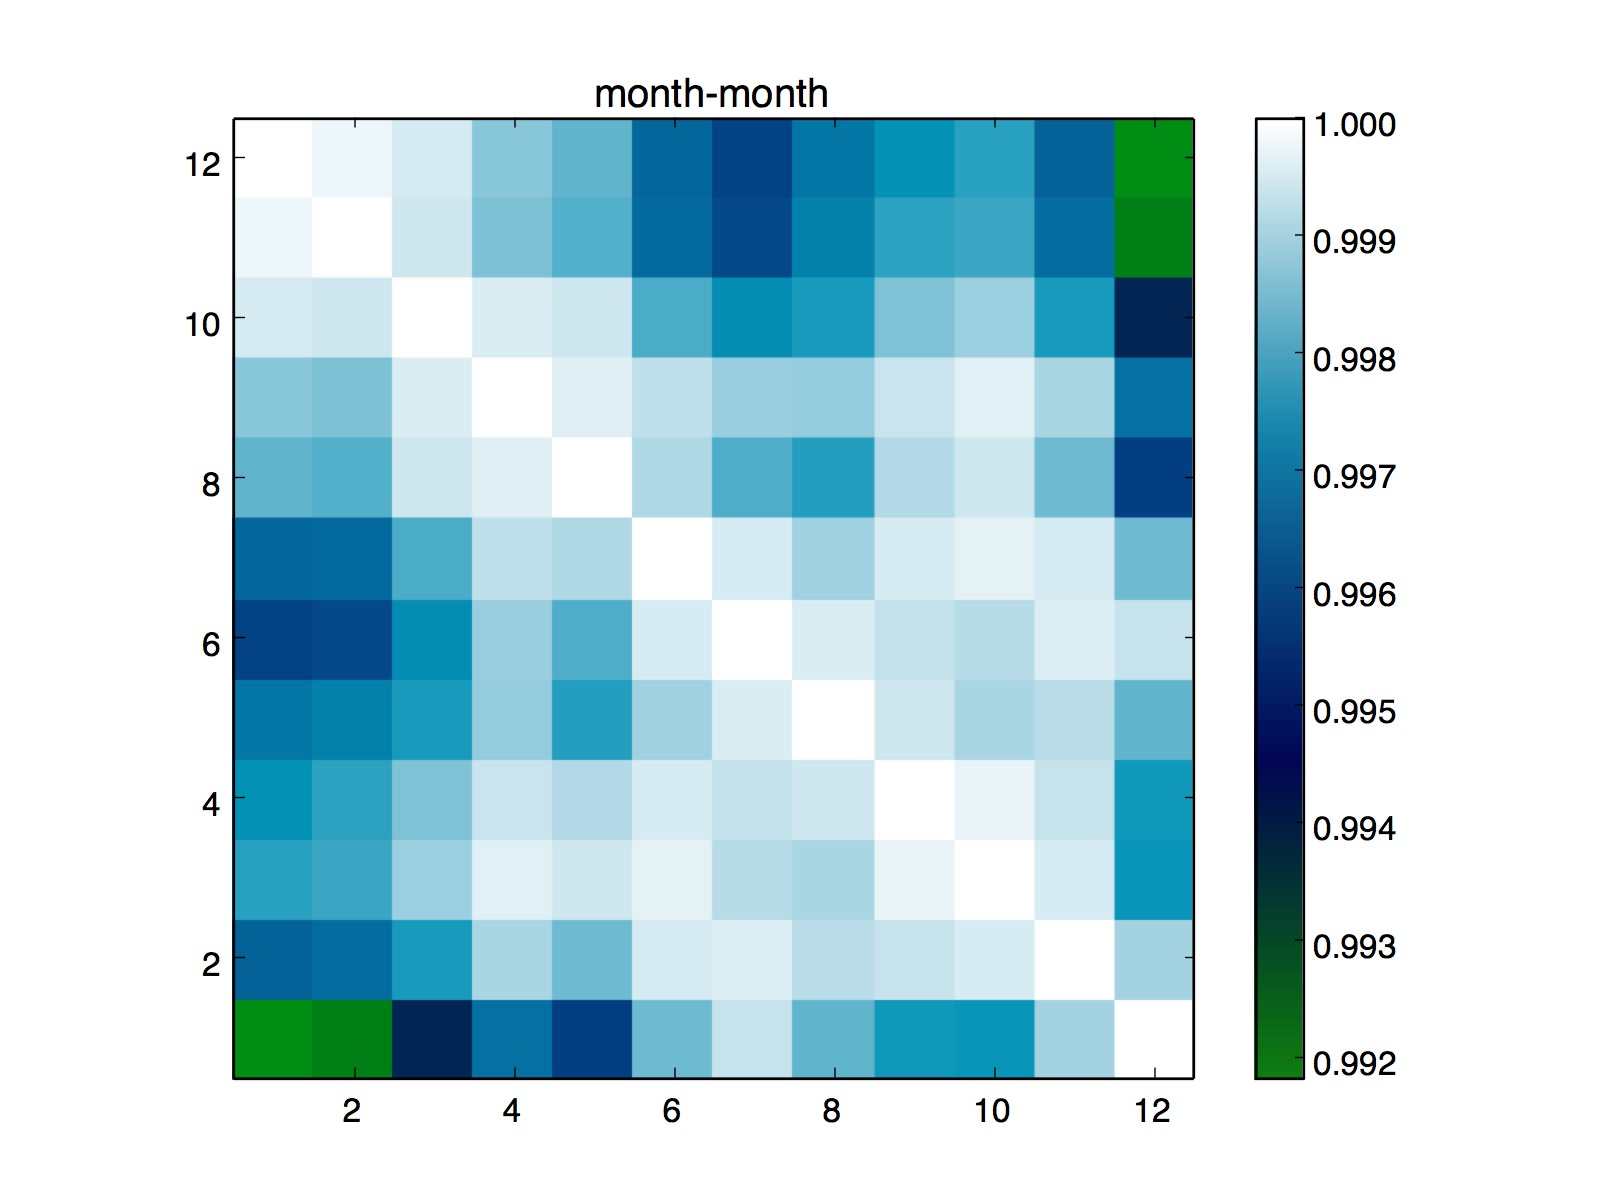
\includegraphics[width=1.0\linewidth]{fig/month_corr}
    \caption{不同月犯罪分布的比较}
    \label{fig:month_corr}
\end{figure}

\begin{figure}[H]
    \centering
    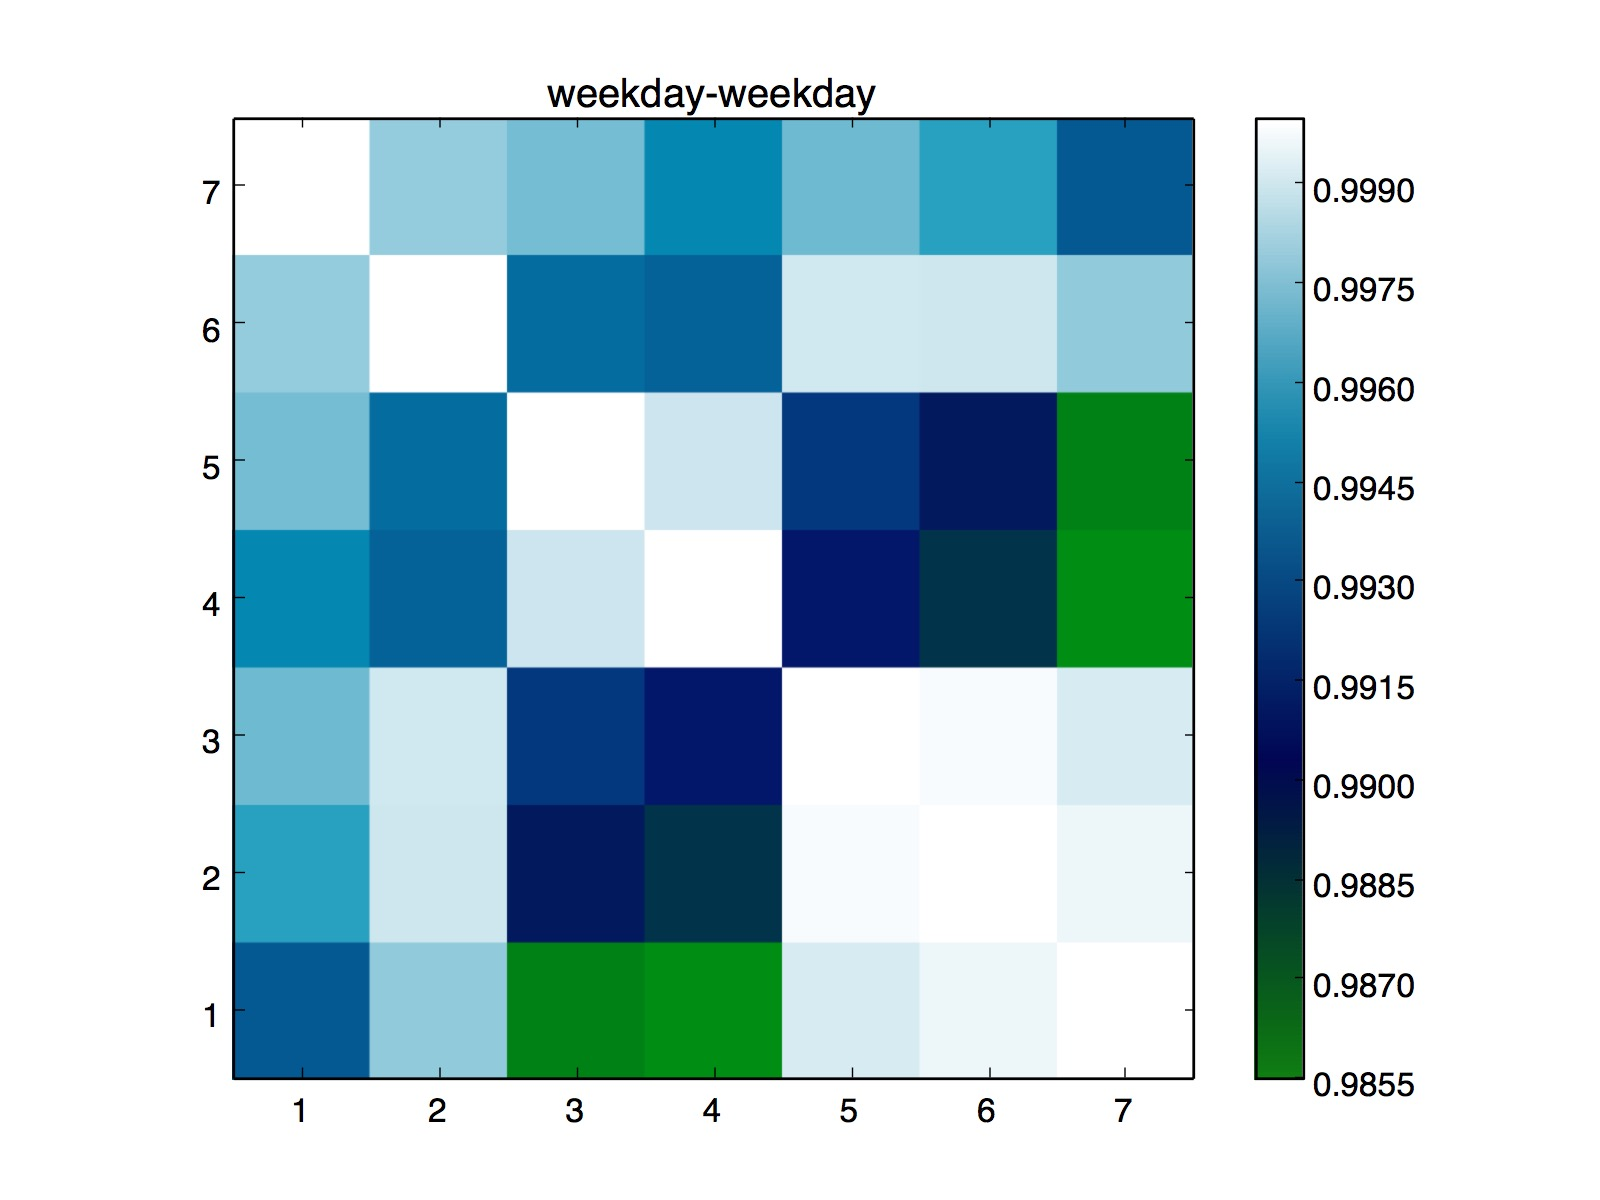
\includegraphics[width=1.0\linewidth]{fig/weekday_corr}
    \caption{每周各天的犯罪分布的比较}
    \label{fig:weekday_corr}
\end{figure}

\subsubsection{细粒度分析方法}

本部分对犯罪分布进行较细粒度的分析,即不仅仅考虑犯罪的总量,也要深入下去对每种不同的犯罪进行考虑。我们既关心不同犯罪类型在时间、空间上的分布是否不同,也关心不同的时间、地点下犯罪类型的分布(即一个$M=38$项的多项分布)是否不同。因此,我们不能仅仅考虑在全部时间段上的计数,而需要对考虑的时间做出一些限制。

\begin{figure}[H]
    \centering
    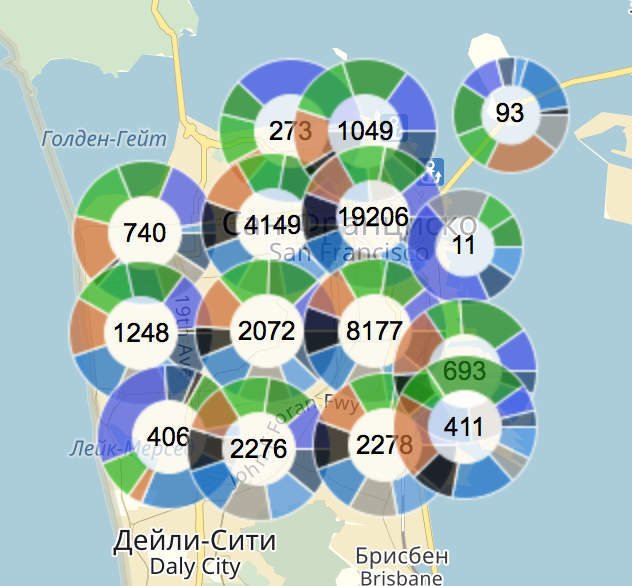
\includegraphics[width=1.0\linewidth]{fig/online_tool}
    \caption{在线分析工具给出的聚类结果}
    \label{fig:online_tool}
\end{figure}

这种细粒度的分析方式如果使用一个数据仓库是比较方便进行的,但数据仓库的实现十分复杂。在Kaggle论坛上,有参赛者公开了一个十分方便的交互式可视化分析工具\footnote{https://www.kaggle.com/tyz910/sf-crime/yet-another-map/notebook,作者Evgeny Ivanov。},可以起到数据仓库的作用。在这个工具中,我们可以对时间进行多种限制:指定日期区间、年份区间,指定某几个星期几和某几个小时。在此基础上,我们可以选定几个犯罪类别。该工具的输出是指定的犯罪类型,在指定的时间限制下,在地图上的聚类结果。同时,在每个聚类中心还会展示这个聚类中每类犯罪的分布情况。这个工具对于我们的探索分析是十分理想的。

图\ref{fig:online_tool}的结果便来自这个工具。图中给出了一定时间范围内,指定的几种犯罪的聚类结果和分布。可以再次验证不同地点的犯罪类型分布是不同的。同样,通过缩小时间范围,并比较不同时间范围的分布,也可以验证之前关于时间的发现,但其实不如我们之前的分析清晰,这里不再罗列。

经过数据可视化分析,我们可以明显地观察出地点和时间信息对于犯罪类型分布的影响。虽然我们发现的一些分布规律不容易直接应用到预测任务之中,但是,这种分析至少让我们可以肯定如果提取适当的特征、选择合适的模型,确实可以通过时间、地点信息推测出犯罪类型。



